%----------------------------------------------------------------------------------------
%	SLIDE 14.
%----------------------------------------------------------------------------------------
\begin{frame}
\frametitle{Párhuzamosítás fizikában}
\framesubtitle{Pythonban}

\begin{exampleblock}{Előfeltételek}
	\begin{itemize}
		\item Pl. a részben már említett \texttt{threading}, \texttt{multiprocessing}, \texttt{joblib}, \texttt{subprocess} stb. csomagok
		\item Több, rendelekzésre álló CPU mag (a Kooplex esetében ez pl. 2 db)
	\end{itemize}
\end{exampleblock}

\begin{figure}
	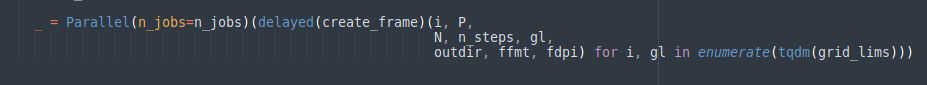
\includegraphics[width=\textwidth]{img/python-joblib.png}
\end{figure}

\begin{figure}
	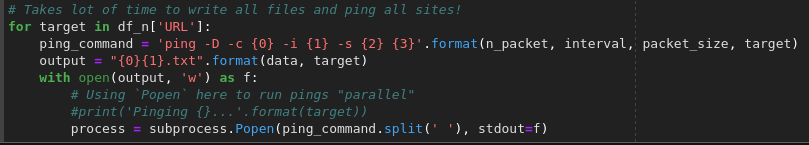
\includegraphics[width=\textwidth]{img/python-subprocess.png}
\end{figure}

\end{frame}